\documentclass[a4paper,10 pt, conference]{article}     %主要指的是文件类型 并指示样式模板为article
\def\allfiles{}     % 加入其它章节文件

% 依赖库
\usepackage{ctex}       % 支持中文
\usepackage{times}      % 支持Arial字体
\usepackage{amsmath}    % 数学公式包
\usepackage{amssymb}    % 字符符号包
\usepackage{graphics}   % 支持图片
\usepackage{subfig}     % 支持子图
\usepackage{caption}    % 支持题注
\usepackage{cite}       % 支持引用文献
\usepackage[numbers]{natbib}    % 引用文献
\usepackage[colorlinks, linkcolor=black]{hyperref}   % 支持超链接

\usepackage{multicol}
\usepackage[top=1in, bottom=1in, left=1.25in, right=1.25in]{geometry}  % 加载包
\usepackage{lscape} %

%文档主体
\begin{document}
    % 标题 作者
    \author{飘散人间的风}     % 作者
    \date{2017年1月12日}      %定义时间
    \title{使用CTEX编写LaTex文件}     %文档标题
    \maketitle %加入上面的的标题作者等信息

    \begin{abstract}
         里面编写摘要
    \end{abstract}

    \textbf{\large Keywords: Keyword A, Keyword B, ...}


    \tableofcontents{}   % 自动生成目录



\section{参考文章}
    \href{http://blog.csdn.net/u014803202/article/details/50410748}{一篇实用的Latex的入门教程}

    \href{http://m.blog.csdn.net/article/details?id=50110329}{(LaTex)CTex的初次使用心得及入门教程}

    《LaTex入门》刘海洋

\ifx\allfiles\undefined
\documentclass[a4paper,10 pt, conference]{article}     %主要指的是文件类型 并指示样式模板为article

\begin{document}
\title{Something in Title}
\author{cohomo@blogbus}
\date{}
\maketitle
\else
\chapter{Chap1's Title}
\fi
\section{First Section}
\section{Second Section}
\ifx\allfiles\undefined
\end{document}
\fi       % 加入其它章节文件,input可以放在导言区和正文区,包含的内容不另起一页;而include只能放在正文区,包含的内容另起一页

\section{文本组织}
    \subsection{字符}
    \subsubsection{转义字符}
    \paragraph{保留字符}

    下面的这些字符是LATEX 的保留字符: \mbox{\# \$ \% \^ \& \_ \{ \} \~ $\backslash$}

    前面加反斜线输出保留字符:\#  \%  \_  \{ \}  \~   \&  \$ 反斜杠比较特殊: $\backslash$

    这下面几个就需要自己用软件编译一下了:
\~{test}   \~{t}{e}{s}{t}
\~{t}\~{e}\~{s}\~{t} \^{}
\^{test}  \textbackslash
\textcopyright \textregistered $^\circ$C
\pounds \dots
\today  \LaTeX{}
\TeX{} \LaTeXe{}



    \subsection{空格缩进}
    \subsubsection{段落控制}
    \paragraph{分节与段落}  文档中使用section与subsection,再下一级用subsubsection类推,合理使用section可以自动生成目录。

    paragraph可添加字符串显示为顶头开始的大写样式,不指定的话默认选定第一个字符。不使用paragraph的段落默认首行缩进2字符。

    \subsubsection{强制空格}
    强制空格种类较多,分为以下几种:

    \begin{enumerate}
    \item 句间空格

    小写字母后面跟标点符号时,该标点符号之后的空格被认为是句间空格。大写字母后面接标点符号,标点符号后的空格会被误认作是词间空格,此时需要在标点符号之前插入 \@ 命令来强制LaTeX将后面的空格作为句间空格处理。例如: as well as I\@ like it. Hence, ...

    \item 词间空格

    书写缩写、省略号等情况下,点 . 之后的空格会被误认为是句间空格。使用 $\backslash$空格 代替普通的半角空格可以强制该空格为词间空格。例如: Yamada et al.\ wrote the report.

    \item 不可分断空格

    用\~代替空格,可使得排版时不会在此处换行。例如 Mr.~Lamport。也可以使用 $\backslash$mbox命令,例: \mbox{Minoru Sakaguchi}。
    \end{enumerate}

    \subsubsection{强制换行}
    源文件中换行和空白符会被忽略,需要强制换行的话使用两种方法:
    \begin{itemize}
    \item 下一行之前插入一个空白行,类似于markdown语法,可以自动缩进
    \item 使用$\backslash$$\backslash$或$\backslash$newline进行强制换行  \hfill \\ 这两种都不会自动缩进,$\backslash$$\backslash$不要放在尾部
    \end{itemize}

    \subsection{列表}
    
    使用$\backslash$ begin\{listtype\}显示列表。 listtype有三种样式。可以使用$\backslash$hfill进行列表标题换行。
    
    \begin{description}
    \item[enumerate] \hfill \\
    使用数字列表
    \item[itemize] \hfill \\
    使用圆点列表
    \item[description] \hfill \\
    使用$\backslash$item[label]指定标签
    \end{description}

    \subsection{合并tex文件}

    参考文章:\href{http://blog.sina.com.cn/s/blog_59cf67260101eat1.html}{Latex之文件拆分及独立编译}

    对应链接:\url{http://blog.sina.com.cn/s/blog_59cf67260101eat1.html}

\section{自动化工具}

    \subsection{引用文献}

    建立一个新文档,将BibTeX类型的引用文字复制到文档,保存文件名为references.bib,保存类型为UTF-8。这个文档专门用来存放参考文献的信息。

    引用go \cite{gostout1992clinical}rivero \cite{rivero2001resistance} 的实验结果。

    在最后需要列出文献列表的地方设定列表显示方式。
    \bibliographystyle{plain}   % 引用样式
    \bibliography{references}   % 使用引用文献的文件名列出文献

    在编译的时候使用XeLaTex编译再用它右边的BiTex(按钮B)编译,再用XeLaTex编译,其他的图片、图表、公式引用也都需要类似编译操作。

    注意:引用文件里*.bib里的\&、\%等字符,需要变成$\backslash$ \&之类。


\section{数学公式}

    \subsection{数学模式}
    \paragraph{进入数学模式} \$...\$是开启行内数学模式,\$\$...\$\$是另起一行的数学模式。\$\$...\$\$会修改默认的公式行间距,有时可能会对文章的整体效果有影响。

    最推荐使用的是equation环境。


    \subsection{公式}
    \paragraph{公式举例}
    希腊字母Greek Letters $\eta$ and $\mu$

    分式Fraction $\frac{a}{b}$

    指数Power $a^b$

    下标Subscript $a_b$

    导数Derivate $\frac{\partial y}{\partial t} $

   向量Vector $\vec{n}$

   加粗Bold $\mathbf{n}$

   对时间的积分To time differential $\dot{F}$

   分式$\Delta = b^2-4ac$
   \[
    x_{1,2} = \frac{-b \pm \sqrt{\Delta}}{2a}
   \]

   矩阵Matrix (lcr分别对应每一列的对其方向)
   \[
     \left[
       \begin{array}{lcr}
         a1 & b22 & c333 \\
         d444 & e555555 & f6
       \end{array}
     \right]
   \]

    公式Equations(\&不同行对其该位置)
    \begin{align}
       a+b&=c\\
       d&=e+f+g
    \end{align}

    \[
       \left\{
         \begin{aligned}
           &a+b=c\\
           &d=e+f+g
         \end{aligned}
       \right.
    \]

    \subsection{引用公式}
    使用$\backslash$ref和{公式的label}进行引用。如下面的公式\ref{abcde}:
    \begin{equation}\label{abcde}
      a+b+c+d+e=f
    \end{equation}


\section{绘制图表}
    \subsection{图片}
    LaTex对jpg、bmp、png等等常见图片都可以支持。插入图片最好放到一个文件下,写清相对当前文件的相对路径。
    \paragraph{简单插入图片}

    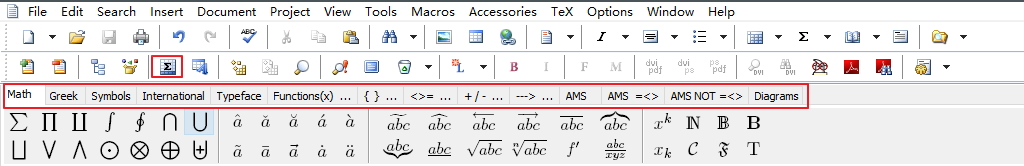
\includegraphics[width=5.00in,height=0.50in]{images/equationHelper.jpg}

    \paragraph{引用图片}

    整体图如图 \ref{label_one-img}所示。
    \begin{figure}[!htbp]
      \centering
      
\includegraphics[width = 0.2\textwidth]{images/image1.jpg}
      \caption{example of one image} \label{label_one-img}
    \end{figure}

  子图\ref{sub1}和子图\ref{sub2}分别进行展示。
    \begin{figure}[!htbp]
      \centering
      \subfloat[first sub-image]{
        
\includegraphics[width = 0.2\textwidth]{images/image1.jpg}
        \label{sub1}
      }
      \qquad
      \subfloat[second sub-image]{
        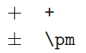
\includegraphics[width = 0.2\textwidth]{images/image2.jpg}
        \label{sub2}
      }
      \caption{combined image}\label{img-together}
    \end{figure}

    \subsection{表格}
    \paragraph{简单插入表格}

    \begin{tabular}{|c|c|}
     aaa & b \\
     c & ddddd\\
   \end{tabular}

    \begin{tabular}{|l|r|}
     \hline
     aaaa & b \\
     \hline
     c & ddddd\\
     \hline
   \end{tabular}

   \begin{center}
     \begin{tabular}{|c|c|}
       \hline
       a & b \\ \hline
       c & d\\
       \hline
     \end{tabular}
   \end{center}

    \begin{table}[h] 表格开始,如果在双栏情况下需要跨栏表格,可以将table改为table*
    \label{表格标示}
    \caption{表格名}
    \begin{center}  %居中
    \begin{tabular}{|c|c|c|c|c|c|}%正式开始:这里的|就表格分成多列,共六列,|cc|也指两列,不过两列中间没有竖线,这里的c指列间是居中放置的
        \hline %指一条长横线,贯穿整个表格,这里是指表格的上框
        1 &2&3 & 4 &5\\ \cline{2-5} %(这里1 2 3 4是表格第一行的内容,而\cline是指此行下面的横线,并不贯穿整个表格,而是从第二个到第五个。而\\指两行的分割)
        &2 &3 & 4 &5\\ \hline %(这里1 2 3 4 5是表格第二行的内容,\hline指一条长横线,贯穿整个表格,这里是指表格的下框)
        %\end{tabular}此表结束
    \end{tabular}
    \end{center}
    \end{table}
    %以上画的表格中上下边框由\hline画出,中间线由\cline,竖线由|确定

   \paragraph{引用表格}
   如表格\ref{表格标示}所示。






    \subsection{浮动体与标题控制}


    \subsection{ 使用色彩}




\end{document}
